\section{直线}
\subsection{直线的方程}
\(y=kx+b\)是一条直线，那么所有的直线方程都可以写作如此吗？\index{直线}
\begin{definition}[直线的倾斜角]
    一般地，给定平面直角坐标系中的一条直线，如果这条直线与\(x\)轴相
    交，将轴绕着它们的交点按逆时针方向旋转到与直线重合时所转的最小
    正角记为\(\theta\)，则称\(\theta\)为这条直线的倾斜角；如果这条直线与\(x\)轴平行或重
    合，则规定这条直线的倾斜角为\(0\du\)。

    从另一个角度来说，倾斜角也可以定义为直线上半部分与\(x\)轴正方向的夹角。
\end{definition}
两点确定一条直线，那么两个点如何求倾斜角？

\begin{theorem}
    在直线上有两点\((x_1,y_1),(x_2,y_2)\)，若\(\)，则倾斜角的正切值即
    为纵坐标变化量与横坐标变化量之比，即
    \begin{equation}
        \tan\theta=\frac{y_1-y_2}{x_1-x_2}
    \end{equation}
    \begin{equation}
        \theta=\arctan\frac{y_1-y_2}{x_1-x_2}
    \end{equation}

    若\(x_1= x_2\)，则\begin{equation}
        \theta=\dfrac{\pi}{2}
    \end{equation}
\end{theorem}
在此出现了倾斜角的正弦值这个量，计算仅仅是纵坐标变化量与横坐标变化量之比，计算起来也比倾斜角更加方便，因此也赋予它一个名字：直线的斜率。
\begin{definition}[直线的斜率]若直线的倾斜角为\(\theta\neq\dfrac{\pi}{2}\)，则定义斜率\(k\)为倾斜角的正切值：
   \begin{equation}
     k=\tan\theta
   \end{equation}
   若\(\theta=\dfrac{\pi}{2}\)，则称直线的斜率不存在。
\end{definition}

\begin{example}
    已知直线\(l\)经过点$A(-1,3)$与$B(2,0)$，求直线\(l\)的斜率$k$与
    项斜角\(\theta\)。
\end{example}
\begin{jie}
    
\end{jie}
\begin{exercise}
  已知直线  $l $ 的斜率为$-\tan \dfrac{\pi}{7} $ ，求 $l $的倾斜角. 
\end{exercise}


结合\(f(x)=\tan x\)在\([0,\pi)\)上的图像，讨论直线斜率的变化。

\begin{center}
    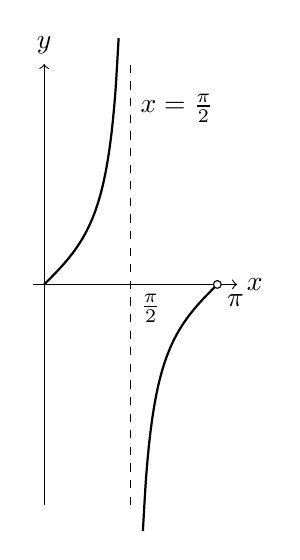
\begin{tikzpicture}[scale=0.7]
      % Grid and axes
      \draw[->] (-0.2,0) -- (3.5,0) node[right] {$x$};
      \draw[ ->] (0,-4) -- (0,4) node[above] {$y$};
      
      % Plotting tan(x)
      \draw[domain=0:0.5*pi-0.22,smooth,variable=\x,thick] plot ({\x},{tan(\x r)});
      \draw[domain=0.5*pi+0.22:pi,smooth,variable=\x,thick] plot ({\x},{tan(\x r)});
      
      % Asymptotes
      \draw[dashed] (pi/2,-4) -- (pi/2,4) node[pos=0.9,right] {$x=\frac{\pi}{2}$};
      
      % Labeling
      \node[below right] at (pi,0) {$\pi$};
      \node[below right] at (0.5*pi,0) {$\frac{\pi}{2}$};
      
      \draw[fill=white] (pi,0) circle [radius=2pt];
    \end{tikzpicture}
\end{center}
%\subsection{直线的方程}
%\subsubsection{直线方程的五种形式}
\begin{example}
    直线的倾斜角为\(\aa\in [\dfrac{\pi}{4},\dfrac{5\pi}{6})\)，求斜率的取值范围。
\end{example}

\begin{definition}[夹角与到角]
    \ 

    两相交直线的夹角 （两直线所成角）是指两直线所成的两对对顶角中，较小的一对角中一个的角；

一条直线\(l_1\)到另一条相交直线\(l_2\)的到角的定义为：\(l_1\)沿着与\(l_2\)的唯一交点逆时针旋转到第一次与\(l_2\)重合
时的有向角，将\(l_1\)称作到角的始边，\(l_2\)称作到角的终边。
\end{definition}
\begin{theorem}
    \begin{equation}
        \tan \theta=\tan \left(\alpha_{2}-\alpha_{1}\right)=\frac{\tan \alpha_{2}-\tan \alpha_{1}}{1+\tan \alpha_{1} \tan \alpha_{2}}=\frac{k_{2}-k_{1}}{1+k_{1} k_{2}}
    \end{equation}
\end{theorem}
\begin{theorem}
    \begin{equation}
        \tan \theta=\left|\frac{k_{1}-k_{2}}{1+k_{1} k_{2}}\right|
    \end{equation}
\end{theorem}
斜率可以非常方便地刻画直线的倾斜程度，但更多的要从题目中尝试去挖掘什么条件刻画了斜率的关系。
\begin{example}
    将直线\(l\)沿着\(y\)轴负方向平移\(a(a>0)\)个单位长度，再沿着\(x\)轴正方向平移\((a+1)\)个单位长度得到
    \(l'\)，则\(l\)的斜率为？
\end{example}
\begin{example}
    设\(A(x_1,y_1),B(x_2,y_2),C(x_3,y_3)\)是函数\(y=x^3\)图像上的任意三个不同的点，
    当\(A,B,C\)三点贡献的时候，求\(x_1+x_2+x_3\)的值。
\end{example}
而斜率不仅仅是刻画直线的倾斜程度，还可以由许多其他的应用。
\begin{theorem}
    \begin{equation}
        d=\sqrt{1+k^2}|x_1-x_2|
    \end{equation}
    \begin{equation}
        d=\sqrt{1+\frac{1}{k^2}}|y_1-y_2|
    \end{equation}
\end{theorem}
此定理的意义在于
\[|x_1-x_2|=\sqrt{(x_1-x_2)^2}=\sqrt{(x_1+x_2)^2-4x_1x_2}\]
\[|y_1-y_2|=\sqrt{(y_1-y_2)^2}=\sqrt{(y_1+y_2)^2-4y_1y_2}\]
最后能够化成关于斜率和韦达定理的形式。

此外，一些形如斜率定义式的式子，往往也可以使用斜率的集合意义求解

\begin{example}
    已知\(x,y\)满足\(y=\dfrac{1}{x}(\dfrac{1}{2}<x<2)\)，求$\dfrac{y+3}{x+2}$的取值范围。
\end{example}
\begin{exercise}
    试比较\(\dfrac{\ln 3}{2},\dfrac{\ln 4}{3},\dfrac{\ln 5}{4}\)的大小。
\end{exercise}
\begin{hint}考虑函数\(\ln (x+1)\)
\end{hint}

\begin{definition}[直线的方向向量与法向量]
    若直线的倾斜角为\(\theta\)，
    
    则直线的方向向量为\( \mathbf{t}\)以及与\( \mathbf{t}\)平行的各个非零向量；
    \begin{equation}
        \mathbf{t}=(\cos \theta,\sin \theta)
    \end{equation}
    直线的方向向量为\( \mathbf{b}\)以及与\( \mathbf{b}\)平行的各个非零向量。
    \begin{equation}
        \mathbf{b}=(\sin\theta,-\cos\theta)
    \end{equation}
\end{definition}
\begin{example}
    若直线\(l\)的一个方向向量为\(\mathbf{a}=\left(\sin\dfrac{\pi}{7},\cos\dfrac{\pi}{7}\right)\)，求直线的倾斜角和一个法向量。
\end{example}

在初中已经熟悉了
形如\(y=kx+b(k\neq 0)\)
的一次函数就是直线，如果允许\(k=0\)，就可以得到
平行于\(x\)轴的直线\(y=b\)。统一起来仍然是\(y=kx+b\)，只不过并不限制\(k\)的取值。
但是仍然有一种直线无法如此表示，即平行于$y$轴的直线\(x=a\)。两种直线在此并没有统一地表达，
原因也很容易看出来：\(y=kx+b\)的\(y\)前面没有参数，总是存在于表达式中，而\(x=b\)中没有\(y\)。

\begin{definition}[直线的一般式方程]
\begin{equation}
    Ax+By+C=0\quad(A^2+B^2\neq 0)
\end{equation}
\end{definition}
\(A^2+B^2\neq 0\)意味着\(A,B\)不同时为\(0\)，亦可以写作\((A,B)\neq (0,0)\)。
\begin{example}
    直线的方程$Ax+By+C=0(A^2+B^2\neq0)$中的\(A,B,C\)满足什么条件时，
直线分别具有如下性质：
\begin{minipage}[t]{0.45\textwidth}
    (1) 过坐标原点； \\
    (2) 与两条坐标轴都相交； \\
    (3) 与$x$轴无交点；
    \end{minipage}
    \hfill
    \begin{minipage}[t]{0.45\textwidth}
    (4) 与$y$轴无交点；\\
    (5) 与$x$轴垂直；\\
    (6) 与$y$轴垂直。
\end{minipage}
\end{example}

\begin{theorem}[一般式方程的方向向量与法向量]
    \ 

    直线\(Ax+By+C=0\)
    \begin{equation}
        \mathbf{t}=(B,-A)
    \end{equation}
    \begin{equation}
        \mathbf{b}=(A,B)
    \end{equation}
    
\end{theorem}


\begin{definition}[直线的斜截式方程]
    \begin{equation}
        y=kx+b
    \end{equation}
    \begin{equation}
        x=my+a
    \end{equation}
\end{definition}


\begin{definition}[直线的点斜式方程]
    \begin{equation}
        y-y_0=k(x-x_0)
    \end{equation}
\end{definition}
\begin{example}
    根据下列条件求直线的点斜式方程；
    
    (1)经过点$A(2,5)$，斜率为$4$；

(2) 经过点$B(-2,2)$，倾斜角为\(30\du \)。
\end{example}

\begin{example}
    已知$P$是直线上一点，且\(\mathbf{t}\)是直线的一个方向向量，
    \(\mathbf{b}\)是直线的一个方向向量，分别根据下列条件求直线的方程：

$(1)\ P(3,5),\ \mathbf{t}=(1,2)$；      

$(2)\ P(1,2),\ \mathbf{b}=(3,4)$。
\end{example}




\begin{definition}[直线的两点式方程]
    
    \begin{equation}
        \frac{y-y_{1}}{y_{2}-y_{1}}=\frac{x-x_{1}}{x_{2}-x_{1}},
    \end{equation}
\end{definition}

\begin{example}
    已知直线经过点$A(2,1),B(3,3)$，求直线的方程，并求直线的截距。
\end{example}
\begin{definition}[直线的截距式方程]
    \begin{equation}
        \frac{x}{a}+\frac{y}{b}=1\quad (ab\neq 0)
    \end{equation}
\end{definition}

\begin{example}
    已知直线\(l\)过点\((3,4)\)，且直线在\(x\)轴和\(y\)轴上的截距相等。求直线的方程。
\end{example}
\begin{exercise}
    已知直线\(l\)过点\(A(-4,-2)\)，且\(A\)是直线\(l\)被两坐标轴截得的线段中线，求直线\(l\)的方程。
\end{exercise}

\begin{theorem}
    直线\(l_1:A_1x+B_1y+C_1=0,l_2:A_2x+B_2y+C_2=0\)，则过\(l_1,l_2\)交点\(P\)的直线方程可写作
    \begin{equation}
        \lambda(A_1x+B_1y+C_1)+\mu(A_2x+B_2y+C_2=0)=0\quad (\lambda^2+\mu^2\neq 0)
    \end{equation}
\end{theorem}

\begin{example} 求出下列直线过的定点。

    （1）\(y=kx+b, b=2k+1\)；
    
    （2）\((2k+1)x+ky+5=0\)。
\end{example}
\clearpage
\subsection{直线的位置关系}
平面上两条直线应该有两种位置关系：平行和相交，当然有时候会把重合算作第三种关系。而其中的
相交还有特殊情况——垂直。接下来使用斜截式和一般式研究直线的位置关系。
\begin{theorem}
    直线\(l_1:A_1x+B_1y+C_1=0,l_2:A_2x+B_2y+C_2=0\)
\begin{enumerate}
    \item 平行
    \begin{equation}
        \frac{A_1}{A_2}=\frac{B_1}{B_2}\neq \frac{C_1}{C_2}
    \end{equation}
    \item 重合
    \begin{equation}
        \frac{A_1}{A_2}=\frac{B_1}{B_2}=\frac{C_1}{C_2}
    \end{equation}
    \item 相交
    \begin{equation}
        \frac{A_1}{A_2}\neq \frac{B_1}{B_2}
    \end{equation}
    \item 垂直
    \begin{equation}
        A_1A_2+B_1B_2=0
    \end{equation}
\end{enumerate}
\end{theorem}


\begin{corollary}
    直线\(l_1:y=k_1+b_1,l_2:y=k_2x+b_2\)
\begin{enumerate}
    \item 平行
    \begin{equation}
        k_1=k_2,b_1\neq b_2
    \end{equation}
    \item 重合
    \begin{equation}
        k_1=k_2,b_1= b_2
    \end{equation}
    \item 相交
    \begin{equation}
        k_1\neq k_2
    \end{equation}
    \item 垂直
    \begin{equation}
        k_1k_2=-1
    \end{equation}
\end{enumerate}
\end{corollary}
\begin{example}
\ 

（1）已知点 $ A(m, 3), B(2 m, m+4), C(m+1,2), D(1,0) $, 且直线 $ A B $ 与直线 $ C D$  平行, 求实数  $m $ 的 值  ；

（2）已知经过点 $ A(-2,0) $ 和点  $B(1,3 a)$  的直线  $l_{1} $ 与经过点 $ P(0,-1)$ 和点  $Q(a,-2 a)$  的直线 $ l_{2} $ 互相垂直, 求实数  $a$  的值为？
\end{example}
\begin{exercise}
    已知直线\(l_1:y=2x+3a,l_2:y=(a^2+1)x+3\)，若\(l_1\pll l_2\)求m的值。
\end{exercise}


\begin{att}
    要时刻注意直线斜率存在与否，以及倾斜角相同的直线是否重合。
\end{att}
\begin{example}
    已知集合\(A=\{(x,y)|\dfrac{y-3}{x-2}=a+1\}\),\(B=\{(x,y)|(a^2-1)x+(a-1)y=15\}\)，若
    \(A\cup B=\varnothing \)，则求\(a\)可能的值。
\end{example}

\begin{definition}[平行直线束]
    \begin{equation}
        y=k_0x+b
    \end{equation}
    \begin{equation}
        A_0x+B_0y+C=0
    \end{equation}
\end{definition}
\begin{definition}[过定点的直线束]
    \begin{equation}
        y-y_0=k(x-x_0)
    \end{equation}
\end{definition}
\begin{example}
    已知直线\(l\)与直线\(y=\dfrac{1}{2}x+4\)互相垂直，直线\(l\)与直线\(y=x+6\)在y轴上截距相等，试求直线
    \(l\)方程。
\end{example}
\clearpage
\subsection{直线相关的距离公式}
\begin{theorem}
    \begin{equation}
          d=\frac{|Ax_0+By_0+C|}{\sqrt{A^2+B^2}}
    \end{equation}
\end{theorem}
\begin{exercise}
    求点\(P_0(-1,2)\)到下列直线的距离\(d\)：
    \begin{enumerate}
        \setlength{\itemsep}{-\itemsep}
        \item \(2x+y-10=0\)；
        \item \(y-3=0\)；
        \item \(x+2=0\)。
    \end{enumerate}
\end{exercise}
\begin{example}
    已知直线 $ l: k x+y+2-k=0 $ 过定点$  M$ ,点 $ P(x, y)$  在直线 $ 2 x-y+1=0$  上, 试求线段$  |M P| $ 的最小值。
\end{example}
\begin{theorem}
    \begin{equation}
          d=\frac{|C_1-C_2|}{\sqrt{A^2+B^2}}
    \end{equation}
\end{theorem}
\begin{exercise}
    求直线\(x+y-1=0\)与直线\(2x+2y+5=0\)之间的距离。
\end{exercise}
在初中就已经熟悉了一点\(P(x,y)\)关于原点、\(x\)轴、\(y\)轴对称后的坐标，后两者可以简单记忆为“关于谁，谁不变”。
\begin{character}
    \ 

 点 $ P\left(x_{0}, y_{0}\right)$ 关于原点的对称点为 $P^{\prime}\left(-x_{0},-y_{0}\right)$ ；

 点  $P\left(x_{0}, y_{0}\right)$  关于  x  轴的对称点为 $ P^{\prime}\left(x_{0},-y_{0}\right)$ ；

  点 $ P\left(x_{0}, y_{0}\right)$  关于  y  轴的对称点为  $P^{\prime}\left(-x_{0}, y_{0}\right) $。
\end{character}

但是如果这个点不再是原点，而是一般的点\((m,n)\)呢？直线也变成了一般式\(Ax+By+C=0\)。
\begin{example}
    求点\(P(x_0,y_0)\)关于点M\((m,n)\)的对称点。
\end{example}
\begin{example}
    求点\(P(x_0,y_0)\)关于直线\(l:Ax+By+C=0\)的对称点。
\end{example}
\begin{example}
    求线\(l:Ax+By+C=0\)关于点M\((m,n)\)的对称点。
\end{example}

\begin{example}
    求线\(l:Ax+By+C=0\)关于点线\(l_0:ax+by+c=0\)的对称点。
\end{example}






\clearpage
\review

\clearpage

\hw
\begin{homework}
    判断下列有关直线方程的命题的真假。
    \begin{enumerate}
        \setlength{\itemsep}{-\itemsep}
        \item 平面上任何一条直线都可以用一个关于\(x,y\)的二元一次方程\(Ax+By+C=0(A^2+B^2\neq 0)\)表示。
        \item 当\(C=0\)时，方程\(Ax+By+C=0(A^2+B^2\neq 0)\)表示的直线过原点。
        \item 当\(A=0,B\neq 0,C\neq 0\)时，方程\(Ax+By+C=0\)表示的直线与\(x\)轴平行。
        \item 任何一条直线的一般式都能与其他四种形式互化。
        \item 斜率相等的直线可以用\(\dfrac{x}{a}+\dfrac{y}{a}=1\)表示。
        \item \(x+my-2=0(m\in\mathbb{R})\)能表示平行于\(y\)轴的直线。
        \item 记过点\(P(1,1)\)，倾斜角为\(\theta\)的直线方程为\(y-1=\tan\theta(x-1)\)。
        \item 过\((x_1,y_1),(x_2,y_2)\)两点的直线方程为\(\dfrac{y-y_{1}}{y_{2}-y_{1}}=\dfrac{x-x_{1}}{x_{2}-x_{1}}\)
    \end{enumerate}
\end{homework}
\begin{homework}
已知$G(-1,0)$为正方形的中心，且这个正方形的一条边所在的直线方程为
$x-3y-5=0$，求这个正方形其他三条边所在的直线的方程。

\end{homework}
\begin{homework}
    已知直线\(l\)经过点$P(2,1)$，且$A(2,3),B(4,—5)$两点到直线的距离相等，求直线\(l\)的方程。
\end{homework}
\begin{homework}

\end{homework}
\begin{homework}求证：
    
    点$  P\left(x_{0}, y_{0}\right)$  关于直线 $ y=x $ 的对称点为 $ P^{\prime}\left(y_{0}, x_{0}\right)$ ；

 点  $P\left(x_{0}, y_{0}\right) $ 关于直线 $ y=-x $ 的对称点为 $ P^{\prime}\left(-y_{0},-x_{0}\right) $；

 点  $P\left(x_{0}, y_{0}\right) $ 关于直线 $ x=m $的对称点为 $ P^{\prime}\left(2 m-x_{0}, y_{0}\right) $；

 点 $ P\left(x_{0}, y_{0}\right) $ 关于直线 $ y=n $ 的对称点为 $ P^{\prime}\left(x_{0}, 2 n-y_{0}\right) $。
\end{homework}
\begin{homework}求证：

直线 $ l: A x+B y+C=0 $ 关于 $ x  $轴的对称直线为  $l^{\prime}: A x+B(-y)+   C=0 .$

直线 $ l: A x+B y+C=0 $ 关于 $ y$  轴的对称直线为 $ l^{\prime}: A(-x)+B y+   C=0 .$

直线 $ l: A x+B y+C=0  $关于直线$  y=x $ 的对称直线为  $l^{\prime}: B x+   A y+C=0 .$

直线 $ l: A x+B y+C=0 $ 关于直线$  y=-x $ 的对称直线为 $ l^{\prime}: A(-y)+   B(-x)+C=0 .$
\end{homework}
\begin{homework}
    
\end{homework}
\begin{homework}
    
\end{homework}
\begin{homework}
    
\end{homework}
\begin{homework}
    
\end{homework}
\begin{homework}
    
\end{homework}
\begin{homework}
    
\end{homework}
\begin{homework}
    
\end{homework}
\begin{homework}
    
\end{homework}
\begin{homework}
    
\end{homework}

\clearpage
